%-----------------------------------------------------------------------
% Functional Programming 4
% John O'Donnell, Wim Vanderbauwhede
% University of Glasgow
%-----------------------------------------------------------------------

\documentclass{beamer}
\usepackage{jtodlecseriesFP4}
%include polycode.fmt
%format alpha = "\alpha"
%format ~> = "\leadsto "

% Identify this presentation
\SetPresentationTitle
  {Reduction, Functions, and Lists}
  {Reduction, Functions, and Lists}
\SetPresentationNumber
  {2}
\SetPresentationDate
  {Week 1-2}
  {Week 1-2}

%-----------------------------------------------------------------------
% Beginning

\begin{document}

\begin{frame}[fragile]
  \PresentationTitleSlide
\end{frame}

\begin{frame}[fragile]
  \frametitle{Topics}
  \tableofcontents
\end{frame}
%-----------------------------------------------------------------------
\begin{frame}[fragile]
\begin{center}
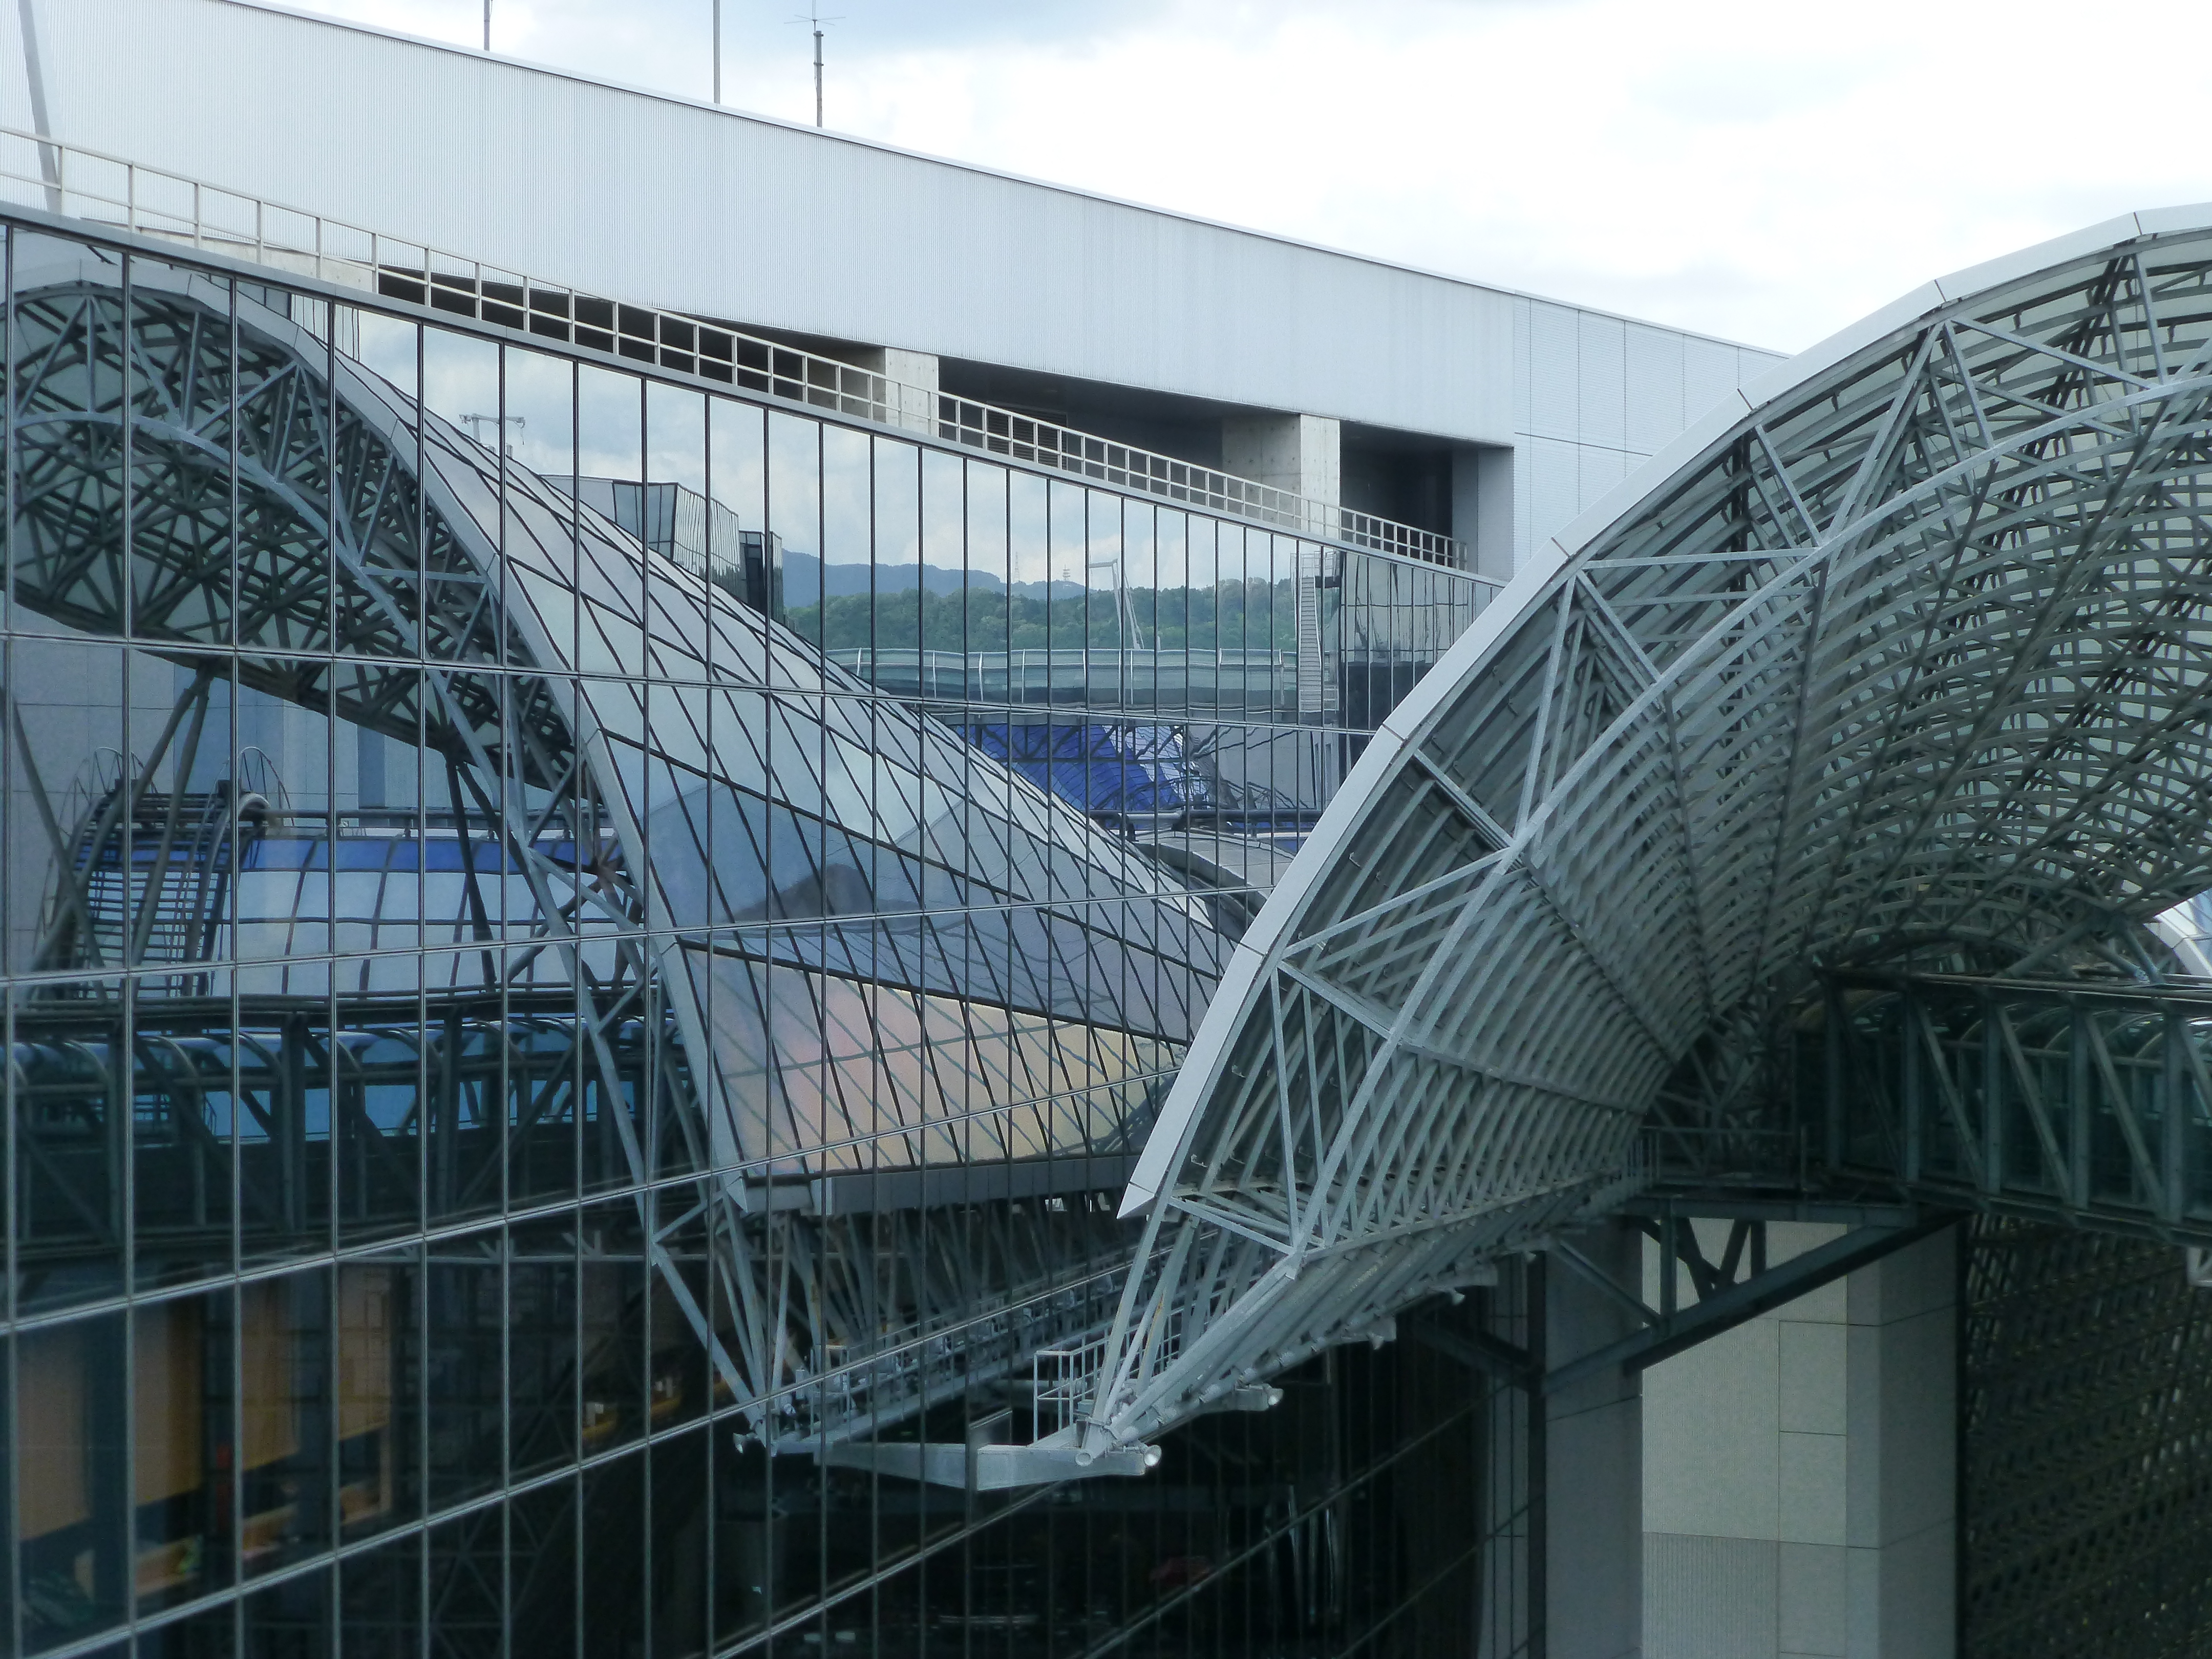
\includegraphics[scale=0.35]
    {figures/jpg/pic02.jpg}
\end{center}
\end{frame}

%-----------------------------------------------------------------------
\section{Reduction}

\begin{frame}[fragile]
\frametitle{Model of program execution}

\begin{itemize}
\item A programmer needs a concrete model for how a program is
  executed.
\item For imperative programs, we can execute statement by
  statement, keeping track of the values of variables (the stack)
  and where we are in the program (the program counter).
\item Functional programs don't have statements!
\item The mechanism for executing functional programs is
  \emph{reduction}.
\end{itemize}

\end{frame}

%-----------------------------------------------------------------------
\begin{frame}[fragile]
\frametitle{Reduction}

An expression is reduced, by simplifying one \emph{reducible
  expression} (called ``redex'').  Each step is called a reduction,
and we'll use \texttt{-- >} to show the result.

\begin{verbatim}
  3 + (4*5)
-- >
  3 + 20
-- >
  23
\end{verbatim}

Reduction is important because it is the sole means of execution of a
functional program.  There are no statements, as in imperative
languages; all computation is achieved solely by reducing expressions.

\end{frame}

%-----------------------------------------------------------------------
\begin{frame}[fragile]
\frametitle{Unique reduction path}


When a reduction is performed, there is only one possible answer.  In
this example, the computation has only one possible path:

\begin{verbatim}
  3 + (5 * (8-2))
-- >
  3 + (5 * 6)
-- >
  3 + 30
-- >
  33
\end{verbatim}

There is only one possible reduction path in that example, because
in each step the current expression contains only one redex.

\end{frame}

%-----------------------------------------------------------------------
\begin{frame}[fragile]
\frametitle{Multiple reduction paths}

If an expression contains several redexes, there will be several
reduction paths.

\vspace{1em}
\begin{center}
%\hbox{
%\fbox
%\hspace{0.5cm}
%\fbox
%}
\end{center}

\end{frame}

%-----------------------------------------------------------------------
\begin{frame}
\frametitle{Result doesn't depend on reduction path!}

A fundamental theorem (the Church-Rosser theorem):

\begin{center}
  \fbox{{\bluetext Every terminating reduction path gives the same result}}
\end{center}

This means that
\begin{itemize}
\item Correctness doesn't depend on order of evaluation.
\item The compiler (or programmer) can change the order freely to
  improve performance, without affecting the result.
\item Different expressions can be evaluated in parallel, without
  affecting the result.  {\redtext \emph{As a result, functional
      languages are leading contenders for programming future
      parallel systems.}}
\end{itemize}

\end{frame}

%-----------------------------------------------------------------------
\section{Functions}

\subsection{Function definitions}

\begin{frame}[fragile]
\frametitle{Function definitions}

\begin{itemize}
\item In Haskell, many functions are pre-defined in a standard
  library called the  \emph{prelude}.% that is automatically available.
%\item In the ghci interpreter, the prompt @Prelude>@ indicates that
%  you have the standard prelude available for use.
\item In due course, we'll learn how to use many of these standard
  functions.
\end{itemize}

\end{frame}

%-----------------------------------------------------------------------
\begin{frame}[fragile]
\frametitle{Defining a function}

\begin{itemize}
\item But the essence of functional programming is defining your own
  functions to solve your problems!
\item A function is defined by an
  \emph{equation}.
\end{itemize}

\begin{verbatim}
f = \x -> x+1  -- lambda function
-- or
f x = x+1 -- named function
\end{verbatim}

This is equivalent to $f(x) = x+1$ in mathematical notation.

\begin{itemize}
\item The left hand side of the equation looks like a variable -- and that's what it is
\item The right hand side is an expression that uses the local variables listen in parentheses and defines the result of the expression.

\end{itemize}

\end{frame}

%-----------------------------------------------------------------------
\subsection{Function application}

\begin{frame}[fragile]
\frametitle{How function application works}

\begin{itemize}
\item A function definition is an equation, e.g. $\tt{f \, =\, \backslash x \rightarrow x+1}$
  \begin{itemize}
  \item The left hand side gives the name of the function;
  \item The right hand side (the ``body'') is an expression giving the
    formal parameters, and  the value of the application.  The expression may use the
    parameters.
  \end{itemize}
\item An application is an expression like \texttt{f 31}, where $31$ is
  the argument.
\item The application is evaluated by replacing it with the body of
  the function, where the formal parameters are replaced by the
  arguments.
\end{itemize}

\end{frame}

%-----------------------------------------------------------------------
\begin{frame}[fragile]
\frametitle{Example of application}

\begin{verbatim}
f  = \x -> x+1
\end{verbatim}

\begin{verbatim}
  f 3
-- > {bind x=3}
  (x+1) where x=3
-- > {substitute 3 for x}
  3+1
-- >
  4
\end{verbatim}

\end{frame}

%-----------------------------------------------------------------------
\subsection{Multiple arguments and results}

\begin{frame}[fragile]
\frametitle{Functions with several arguments}

A function with three arguments:

\begin{verbatim}
add3nums = \x y z -> x + y + z
\end{verbatim}

To use it,

\begin{verbatim}
  10 + 4* add3nums 1 2 3
= {put extra parenthese in to show structure}
  10 + ( 4* (add3nums 1 2 3) )
-- >
  10 + (4*(1+2+3) )
-- >
  10 + (4*6)
-- >
  10 + 24
-- >
  34
\end{verbatim}

\end{frame}


%-----------------------------------------------------------------------
\section{Lists}
\begin{frame}[fragile]
\frametitle{Lists}

\begin{itemize}
\item A list is a single value that contains several other values.
\item Syntax: the elements are written in square parentheses,
  separated by commas.
\end{itemize}

\begin{verbatim}
['3', 'a']
[2.718, 50.0, -1.0]
\end{verbatim}

\end{frame}

%-----------------------------------------------------------------------
\begin{frame}[fragile]
\frametitle{Function returning several results}

\begin{itemize}
\item Actually, a function can return only one result.
\item However, lists allow you to package up several values into
  one object, which can be returned by a function.
\item Here is a function $minmax$ that returns both the smaller and
  the larger of two numbers:
\end{itemize}

\begin{verbatim}
minmax = \x y -> [min x y, max x y]
\end{verbatim}

\begin{verbatim}
minmax 3 8  -- > [3,8]
minmax 8 3  -- > [3,8]
\end{verbatim}

\end{frame}


%-----------------------------------------------------------------------
\begin{frame}[fragile]
\frametitle{The elements are evaluated}

You can write a constant list

\begin{verbatim}
mylist = [2,4,6,8]
\end{verbatim}

But the elements can be expressions, which are evaluated.  Suppose
you define:

\begin{verbatim}
answer = 42
yourlist = [7, answer+1, 7*8]
\end{verbatim}

Then

\begin{verbatim}
  yourlist
-- >
  [7, 43, 56]
\end{verbatim}

\end{frame}
%-----------------------------------------------------------------------
\subsection{Constructing lists}

\begin{frame}[fragile]
\frametitle{Append: the $(++)$ operator}

\begin{itemize}
\item The $(++)$ operator  takes two existing lists, and gives
  you a new one containing all the elements.
\item The operator is pronounced \emph{append}, and written as two
  consecutive + characters.
\end{itemize}

\begin{verbatim}
  [23, 29] ++ [48, 41, 44]
-- >
  [23, 29, 48, 41, 44]
\end{verbatim}

A couple of useful properties:

\begin{itemize}
\item The length of the result is always the sum of the lengths of
  the original lists.
\item If $xs$ is a list, then $[] ++ xs = xs = xs ++ []$.
\end{itemize}

\end{frame}

%-----------------------------------------------------------------------
\begin{frame}[fragile]
\frametitle{Sequences}

\begin{itemize}
\item Sometimes it's useful to have a sequence of numbers.
\item In standard mathematical notation, you can write $0, 1,
  \ldots, n$.
\item Haskell has a sequence notation for lists.
\item Write the sequence in square brackets, with start value, the
 operator \texttt{..}, and end value.
  \begin{itemize}
  \item \texttt{[0 .. 5] \-- > [0,1,2,3,4,5]}
  \item \texttt{[100 .. 103] \-- > [100,101,102,103]}
  \end{itemize}
\item The elements are incremented by 1 
%or -1.  But you can achieve an
%  arbitrary increment by saying \texttt{by n}.
%  \begin{itemize}
%  \item \texttt{[1 to 20 by 2] \-- > [1,3,5,7,9,11,13,15,17,19]}
%  \item \texttt{[0 to -5] \-- > [0,-1,-2,-3,-4,-5]}
%  \end{itemize}
\end{itemize}

\end{frame}

%-----------------------------------------------------------------------
\begin{frame}[fragile]
\frametitle{Sequences aren't limited to numbers}

\begin{itemize}
\item There are many \emph{enumerable types} where there is a natural
  way to increment a value.
\item You can use sequences on any such type.
\item Characters are enumerable: there is a successor to each
  character.
  \begin{itemize}
  \item \texttt{['a' .. 'z'] \-- > ['a','b','c','d','e','f','g','h','i','j','k',\\
  'l','m','n','o','p','q','r','s','t','u','v',\\
  'w','x','y','z']}
  \item \texttt{['0' .. '9'] \-- > ['0','1','2','3','4','5','6','7','8''9']} is a list of characters
    (which happen to be the digit characters)
  \item \texttt{[0 .. 9] \-- > [0,1,2,3,4,5,6,7,8,9]} is a list of numbers
  \end{itemize}
\end{itemize}

\end{frame}

%-----------------------------------------------------------------------
\begin{frame}[fragile]
\frametitle{List comprehensions}

\begin{itemize}
\item A list comprehension is a high level notation for specifying
  the computation of a list
\item The compiler automatically transforms a list comprehensions
  into an expression using a family of basic functions that operate
  on lists
\item List comprehensions were inspired by the mathematical
  notation \emph{set comprehension}.
\item Examples of set comprehensions:
  \begin{itemize}
  \item A set obtained by multiplying the elements of another set
    by 3 is $\{3 \times x \;|\;x \leftarrow \{1, \ldots, 10\}\}$.
  \item The set of even numbers is $\{2 \times x \;|\; x
    \leftarrow N \}$.
  \item The set of odd numbers is $\{2 \times x + 1 \;|\; x
    \leftarrow N \}$.
  \item The cross product of two sets $A$ and $B$ is $\{(a,b) \;|\;a \leftarrow A, b \leftarrow B\}$.
  \end{itemize}
\end{itemize}

\end{frame}

%-----------------------------------------------------------------------
\begin{frame}[fragile]
\frametitle{Examples of list comprehensions}

\begin{verbatim}
  [3*x | x <- [1..10]]
-- >
  [3,6,9,12,15,18,21,24,27,30]
\end{verbatim}

\begin{verbatim}
  [2*x | x <- [0..10]]
-- >
  [0,2,4,6,8,10,12,14,16,18,20]
\end{verbatim}

\begin{verbatim}
  [2*x + 1 | x <- [0..10]]
-- >
  [1,3,5,7,9,11,13,15,17,19,21]
\end{verbatim}

\begin{verbatim}
  [[a,b] | a <- [10,11,12] , b <- [20,21]]
-- >
  [[10,20],[10,21],[11,20],[11,21],[12,20],[12,21]]
\end{verbatim}

\end{frame}

%%-----------------------------------------------------------------------
\subsection{Operating on lists}

%-----------------------------------------------------------------------
\begin{frame}[fragile]
\frametitle{Indexing a list}

\begin{itemize}
\item We can index a list by numbering the elements, starting with
  0.
\item Thus a canonical form of a list with $n$ elements is $[x_0,
  x_1, .. x_{n-1}]$.
\item The $!!$ operator takes a list and an index, and
  returns the corresponding element.
  \begin{verbatim}
[5,3,8,7]  !! 2    -- > 8
[0 .. 100]  !! 81  -- > 81
['a'..'z'] !! 13  -- > 'n'
  \end{verbatim}
\item If the index is negative, or too large, \emph{undefined} is returned.
\item For robust programming, we need to ensure either that all
  expressions are well defined, or else that all exceptions are
  caught and handled.
\item Later, we'll look at how to follow both of those approaches.
\end{itemize}

\end{frame}

%-----------------------------------------------------------------------
\begin{frame}[fragile]
\frametitle{\emph{head} and \emph{tail}}

\begin{itemize}
\item There are standard library functions to give the head of a
  list (its first element) or the tail (all the rest of the list)
\item The result of applying $head$ or $tail$ to the empty list is
  \emph{undefined}.


\begin{verbatim}
head :: [a] -> a
head [4,5,6] -- > 4
tail :: [a] -> [a]
tail [4,5,6] -- > [5,6]
\end{verbatim}


\item Recommendation:  avoid using $head$ and $tail$, because you
  want to avoid undefined values so your programs are robust.
  Unless you're doing something really sophisticated, you're better
  off with pattern matching.  There are, however, some cases where they are appropriate.
\end{itemize}

\end{frame}


\end{document}
